
%=============================================================================
%  File:          main.tex
%  Author:       Roman Patscheider und Fabian Hilti
%                Automatik Control Lab, ETH Zurich, Switzerland
%                
%  Content:      Template for student reports
%  Creation:     11 Jan 2001
%  Last change:  continuous ...
%=============================================================================
\newif\ifpdf
\ifx\pdfoutput\undefined
  \pdffalse
\else
  \pdfoutput=1
  \pdftrue
\fi

\ifpdf
\documentclass[11pt,            % 11pt Font
               a4paper,         % a4-Paperformat
               twoside,         % twoside
               fleqn,           % Equations appear flush left
               pdftex
               ]{report}
\else
\documentclass[11pt,            % 11pt Font
               a4paper,         % a4-Paperformat
               twoside,         % twoside
               fleqn,           % Equations appear flush left
               openright        % Chapters begin on odd (right) page
              ]{report}
\fi


\ifpdf
     \usepackage[colorlinks,hyperindex]{hyperref}% generates colored links
                                                 % in pdf file
     \usepackage[pdftex]{graphicx}
     \DeclareGraphicsExtensions{.png, .jpg, .pdf}
     \graphicspath{{pictures/}}
\else
     \usepackage[dvips]{graphicx}
     \DeclareGraphicsExtensions{.eps}
     \graphicspath{{pictures/}}
\fi

\usepackage[T1]{fontenc}        % T1-Fontcoding, auch notwendig
                                % um mit Umlauten ,, arbeiten zu koennen
\usepackage{ae}                 % Almost european computer modern font
                                % Zur Erstellung von pdf-Files
\usepackage[english]{babel}      % Package for multilingual style options
\usepackage{fancyhdr}           % Package for customizing page layout
\usepackage{ETHkopfTwo}         % ETH Style Title page
\usepackage{AufgTwo}            % Formatiert die Aufgabenstellung
\usepackage{verbatim}           % Package for including files
\usepackage[final]{pdfpages}	% Bindet PDF ein
\usepackage{amsmath}
\usepackage{placeins}

%=============================================================================
% Layout Header and Footer
%=============================================================================

\pagestyle{fancy}
% with this we ensure that the chapter and section
% headings are in lowercase.
\renewcommand{\chaptermark}[1]{\markboth{\thechapter\ #1}{}}
\renewcommand{\sectionmark}[1]{\markright{\thesection\ #1}}
\fancyhf{}                           % Delete all current settings
                                     % for header and footer
\fancyhead[LE,RO]{\bfseries\thepage} % Pagenumber aligned left on odd pages
                                     % Pagenumber aligned right on
                                     % even pages
\fancyhead[LO]{\nouppercase{\bfseries\rightmark}}
\fancyhead[RE]{\nouppercase{\bfseries\leftmark}}
\renewcommand{\headrulewidth}{0.5pt}
\renewcommand{\footrulewidth}{0pt}
\addtolength{\headheight}{1.6pt}     % Make space for headrule
\fancypagestyle{plain}
{
\fancyhead{}                         % Get rid of headers on plain pages
\renewcommand{\headrulewidth}{0pt}   % Get rid of headerline on plain pages
}

%=============================================================================
% Pagelayout
%=============================================================================

\addtolength{\headwidth}{1.2cm}
\addtolength{\textwidth}{1.2cm}
\addtolength{\evensidemargin}{-1.2cm}
\addtolength{\oddsidemargin}{-0cm}


%=============================================================================
% Numbering depth for headings
%=============================================================================
\setcounter{secnumdepth}{3} % Within document
\setcounter{tocdepth}{3}    % Within table of contents

%=============================================================================
% New commands
%=============================================================================

% These commands may be used instead of the built-in commands of LaTeX
% for creating your equations
\newcommand{\be}{\begin{equation}}          % Abbreviation
\newcommand{\ee}{\end{equation}}
\newcommand{\bea}{\begin{eqnarray}}
\newcommand{\eea}{\end{eqnarray}}


%Command clear used to produce empty page without header and footer
%in case of a twoside report where new chapters always begin on odd pages
\ifpdf
   \newcommand{\clear}{}
\else
   \newcommand{\clear}{\newpage{\pagestyle{empty}\cleardoublepage}}
\fi


\frenchspacing

%=============================================================================
% Begin of document
%=============================================================================

\begin{document}
    
\begin{titlepage}
   \pagestyle{empty}
   \topmargin=1.2cm
   \ETHkopfTwo{Automatic Control Laboratory}{Prof. Roy Smith}{Springterm 2012}
   \noindent
   \rule{\textwidth}{0 mm}\\



\begin{center}
\Large \bfseries Semester Thesis\\
\vspace{1cm}
\Huge \bfseries Sensor Fusion / State Estimation for a Kite Power Plant

\vspace{1cm}



%Titelbild einfgen
\vspace{0.1cm}%Grsse verndern zur Positionierung des Bildes

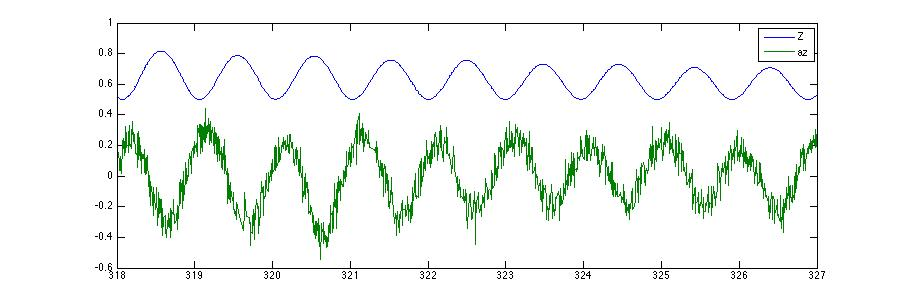
\includegraphics[width=0.75\textwidth]{pictures/titelbild.jpg}
\end{center}

 \vspace{1cm}

    \noindent
    \rule{\textwidth}{1 mm}\\
    \noindent
    \bfseries \large
    \makebox[0.5\textwidth][l]{\emph{Authors:}}
    \makebox[0.49\textwidth][r]{\emph{Advisers:}}

    \vspace{0.2 cm} \noindent
    \makebox[0.5\textwidth][l]{Roman Patscheider}
    \makebox[0.49\textwidth][r]{Aldo Zgraggen}
    \makebox[0.5\textwidth][l]{Fabian Hilti}
    \makebox[0.49\textwidth][r]{Corey Houle}
    \makebox[0.5\textwidth][l]{}
    \makebox[0.49\textwidth][r]{}
    \makebox[0.5\textwidth][l]{}
    \makebox[0.49\textwidth][r]{}
    \mdseries \normalsize


\end{titlepage}

\clear
    \pagenumbering{roman}

    %\include{Vorwort}
\clear
    \tableofcontents
\clear
    \listoffigures % Creates list of all figures used in document
%\clear
    %\listoftables  % Creates list of all tables inserted
\clear
    \chapter*{Abstract}
\addcontentsline{toc}{chapter}{Abstract}

Bla Bla Bla













\clear


% Split your document e.g. chapterwise and rejoin the chapters
% to a single documentation with the \include-Command
    \pagenumbering{arabic}
    \chapter{Introduction}\label{cha1}
\section{Kite Power in General and the SwissKitePower Project}
At a time when windmills were already quite commonly used for power generation, Loyd came up with the idea to use kites to convert wind energy to electricity.  In 1980 he wrote a seminal paper exploring the possibility of generating electrical power using the pulling force of tethered airfoils, i.e., kites \cite{loyd1980}. He describes his concept as follows:
\begin{quote} A kite's aerodynamic surface converts wind energy into motion of the kite. This motion may be converted into useful
power by driving turbines on the kite or by pulling a load on the ground. [...] Not simply facing into the wind, such kites would fly a closed path downwind from the tether point. The kite's motion would be approximately transverse to the wind, in the same sense that a wind turbine's blade moves transverse to the wind. The crosswind airspeed of a kite with this trajectory is increased above the wind speed by the lift-to-drag ratio L/D. The resultant aerodynamic lift is sufficient to support a kite and to generate power. \cite{loyd1980}\end{quote}
Today, several research groups around the world are investigating this subject and working on prototypes. For example the University of Torino have already tested a prototype \cite{canale2006} and Massimo Ippolito has founded a company named KiteGen that is also located in Torino. At the University of Delft the group of Prof. Dr. Wubbo Oeckels is developing kites to produce energy with "Laddermills" \cite{schmehl2012} and at the K. U. Leuven the group of Prof. Moritz Diehl is working on the Highwind project \cite{geebelen2012}. Furthermore the SkySails company is already using wind power to pull large cargo ships \cite{erhard2012} and Ampyx Power, a spin-off from T.U.Delft is working on their PowerPlane device.

In Switzerland the research efforts are coordinated in the SwissKitePower Project \cite{skp}. SwissKitePower is a collaborative research and development project between FHNW (University of Applied Sciences Northwestern Switzerland), ETHZ (Swiss Federal Institute of Technology Zurich), EMPA (Swiss Federal Laboratories for Materials Testing and Research) and Alstom Switzerland AG. The goals of the project are to develop 'novel wind energy extraction technology' using tethered airfoils, or kites, and to promote this innovative new technology to the world.

\section{Related Work}
There are many publications on the topic of IMU/GPS data fusion for navigation purposes. As a starting point of our work we used the Master Thesis of Andr\'{a}s H\'{e}jj "Kalman-filter based position and attitude estimation algorithms for an Inertial Measurement Unit" \cite{hejj}. In an other Master project at the University of Southern Denmark Ushanthan Jeyabalan implemented a Kalman Filter using a spherical pendulum model \cite{ushanthan}.
Several other publications investigated the use of a Kalman Filter for IMU/GPS data fusion in different applications. Sukkarieh applied it to land vehicles \cite{sukkarieh1999}, Kim used it for unmanned areal vehicles in highly dynamic flight situations \cite{kim2006} and Crassidis used a Sigma Point Kalman Filter and compared it to an EKF. This list of course is not exhaustive. A much broader overview over the various approaches to multisensor data fusion in target tracking can be found in the survey article of Smith and Singh \cite{smith2006}.
 


\section{Motivation and Methods}
In order to successfully implement a control algorithm on a kite, it is essential that a precise and fast position estimation is available. Due to the slow update rate of the GPS units and their limited reliability, a Kalman Filter will be used to integrate IMU measurements, which consist of acceleration, rate of turn and magnetic field, with the GPS position and velocity estimations. A standard Kalman Filter, one that could also be used in an airplane for example, assumes no knowledge aboout forces acting on the body. Such an estimator will already enhance the position estimation from the raw GPS input since it incorporates more measurements.  However, a kite can only move on a restricted surface due to it being thethered to the groundstation. An extended Kalman Filter could take advantage of that knowledge and further improve the estimator's performance. Further integrating an aerodynamical model of the kite could give more information about the forces acting on it and would reduce the estimator's dependency on precise sensor output.  

In order to be able to compare the performance of the different estimators, it is neccessary to know the exact location and orientation of the kite at all times. In practice it is nearly impossible to obtain such a ground truth for a kite flying around in the air. Therefore we decided to investigate the benefits of an accurate physical model on the performance of a Kalman Filter using box suspended by a string. (See figure ...) This setup can be modeled as a spherical pendulum which has the advantage that all the forces acting on it are known.  In addition, we are able to test the algorithms indoors using a Vicon System (add reference!!) that gives us a very accurate ground truth of the box's position and orientation. Since there is obviously no GPS reception indoors, the GPS output needs to be simulated using the Vicon's position output, reducing its frequency and adding an appropriate level of noise.



 % TeX includes file Chapter1.tex
\clear
    \chapter{IMUs}\label{cha2}

For estimating the kite's state measurements from different sensors are needed. In so called inertial measurements units (IMU)  several sensors are embedded. The most important difference between the the IMUs are in what sensors are embedded, with which rate do they provide the data, what is their range and sensitivity and how much signal processing is already done by the IMU.
The Swiss Kite Power Project has the following options of IMUs to choose:

\begin{description}
\item[MTi-G]
The MTi-G development kit is a commercial product from the Dutch company Xsens. The unit has an accelerometer, gyroscope, magnetometer, pressure sensor and GPS with antenna included. It exist two output data formats. It can be chosen wether the output is raw data or calibrated data. The calibrated data from the sensors without GPS gives the data in $[m/s^2]$ and takes a offset calibration test into account. In addition to that is the GPS data processed with an Extended  Kalman Filter in the calibrated output mode.

\item[PX4]
The PX4 is a open-source/open-hardware IMU used and developed by the PIXHAWK Project of the Computer Vision and Geometry Lab of ETH Zurich. The unit contains a temperature and pressure sensor, an accelerometer, a gyroscope and a magnetometer. The IMU additionally provides a counter for each sensor output. The output of the sensors is raw data. In the estimation algorithm( …....label estimation chapter …....) only the embedded accelerometer a BMA180 from Bosch (…..DataSheetAppendix.....), the gyroscope a L3GD20 from STMicroelectronics (…..DataSheetAppendix...) and the magnetometer a HMC5883L from Honeywell (….DataSheetAppendix...) is used.

\item[x-IMU]
The x-IMU is a product of the company x-io Technologies. It has as well a temperature sensor, a accelerometer, a gyroscope and a magnetometer. The setting of the x-IMU was done by the FHNW. It provides only raw data. The data sheets of the sensors can be found in the (…..APPENDIX.....).
\section{Centrifue Test}
There are several performance requirements on an IMU installed on a kite. One of them is the dependency on g-loads because on a kite several g loads can appear. Therefore a centrifuge test was carried out in corporation with the Fachhochschule Nordwestschweiz (FHNW)
\subsection{Set-up}
Set-Up
The setting of the centrifuge is described in (…..Figure.....). It is provided by the FHNW. A arm is rotated by a motor. The IMUs are set into a box at the end of the arm. The sensors are put next to each other to have the almost the same measurements in all sensors. The Box can be seen on the picture in (….Figure....). Obviously is the motion of the box describing a circle with a radius (he distance between the center and the  center of the box) of $0.75 m$. The motor is able to rotate the arm with a velocity of about $10 m/s$. With formula $a=\omega*r^2$ we get maximum acceleration of about $8 g$. There is no software for the data collection of the measured velocity implemented. Therefore we have no ground truth to compare the sensor data with. The motor is driven in order to have 5 steps between $1.62 g$ and $7.8 g$ $(ca. 1.6 g; 2.4 g 3.7 g; 5.4 g; 6.9 g; 7.8 g)$ of centripetal acceleration.
The PX4 and Xsens are connected together. Both, the PX4 and the Xsens measurements are written on the SD card which is attached on the PX4 Unit. The timestamp is taken from the GPS clock for the Xsens as well as for the PX4 sensor data at the time when they are written on the SD card. This results in easy and accurate synchronization between the two IMUs. To get the time synchronized with the third IMU, the x-IMU is synchronized to the computer's time. Additionally the 3 sensors are hit for having a estimation of how accurate the synchronization is.
\subsection{Result}
The raw data from the x-IMU is scaled by Raphael Mueller bringing it in the common units $m/s^2$ for the accelerometer, $deg/s$ for the gyroscope and gauss for the magnetometer.
The PX4 was set by the group of the PixHawk Project. How the output of the sensors have to be scaled to bring them in the required units is shown in (….table...). The scale factor describes by how much the output has to be multiplied to get the data converted in the units described in 4th row.
\subsection{Conclusion}
All IMUs work in the same range of noise level. With an increasing rotational velocity and therefore a higher centripetal acceleration, the average error is increasing in all sensors, except in the magnetometer. There could not be found a noise acceleration dependency. 
In a next experiment also the recording of rotational velocity should be carried out in order to generate a ground truth to compare the it with the IMU datas. It can then be made some more observations to compare the quality of the sensors with each other. Finally the sensitivity of the accelerometer of the PX4 unit should be set in a way to be able to observe the whole range or the applied and tested centripetal acceleration.


\clear
    \chapter{State Estimation}\label{cha3}
\section{Basics of the Extended Kalman Filter}
\section{State Estimation Model}
\section{Sensor Estimation Model}
\section{Covariances, Outage}

\clear
    \chapter{Results - Vicon Test}\label{cha4}
\section{Set up}
\section{Evaluation}
\subsection{short vs long radius}
\subsection{Outage and Sensor rate}
\subsection{Pixhawk vs Xsens}



\clear
    \chapter{Conclusion}\label{cha}

\clear
    %\include{Zusammenfassung}
\clear
    %\include{Ausblick}
\clear
    %Bibliography
    \bibliographystyle{unsrt}
    \bibliography{bibliography}
\clear
%\begin{appendix}
    %Appendix
    \appendix
    \chapter{Data Sheets of the PX4 sensors}\label{ds}
%{Data Sheet of the Accelerometer from the PX4}
\section{Data Sheet of the Accelerometer}\label{ds_acc}
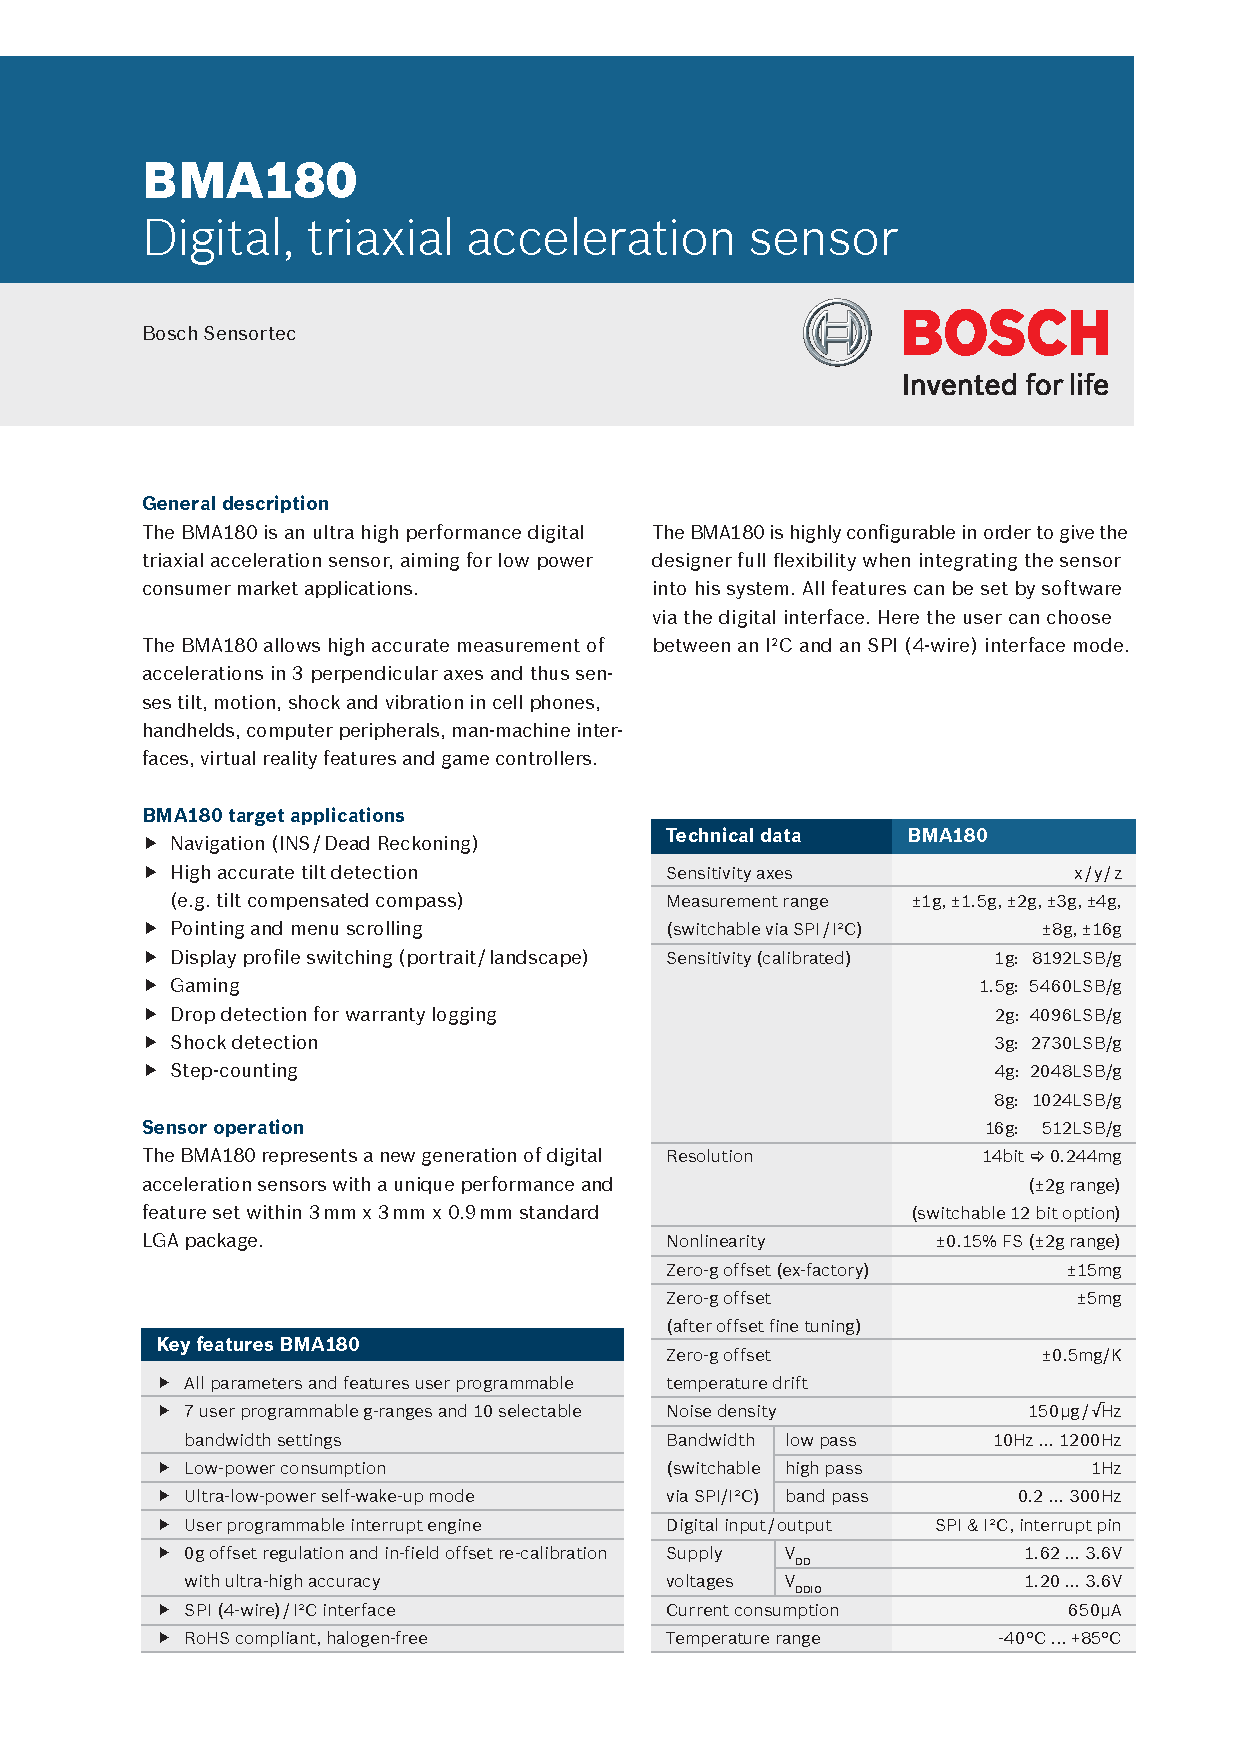
\includepdf[pages=-]{appendix/acc-BST-BMA180-FL000-03.pdf}
\section{Data Sheet of the Gyroscope}\label{ds_gyro}
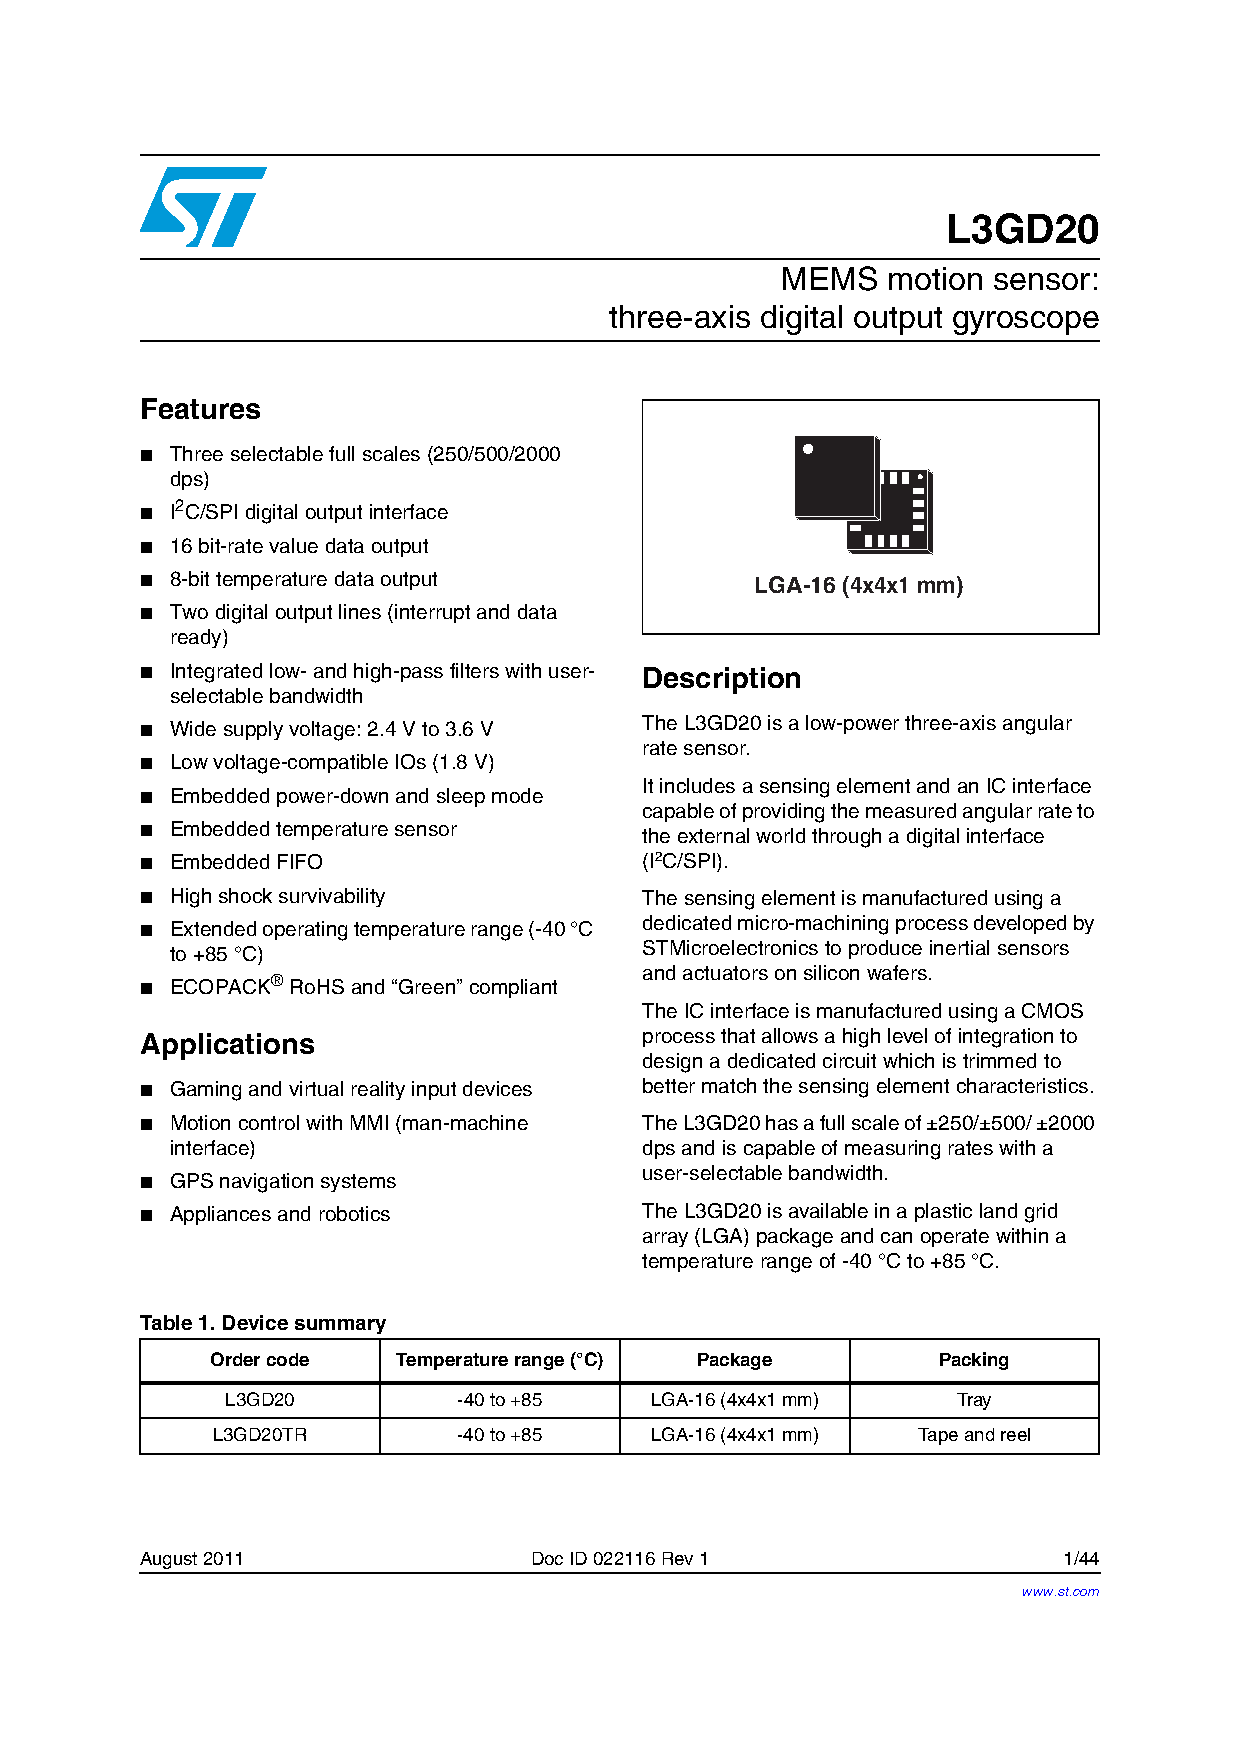
\includepdf[pages=-]{appendix/gyro_px4.pdf}
\section{Data Sheet of the Magnetometer}\label{ds_mag}
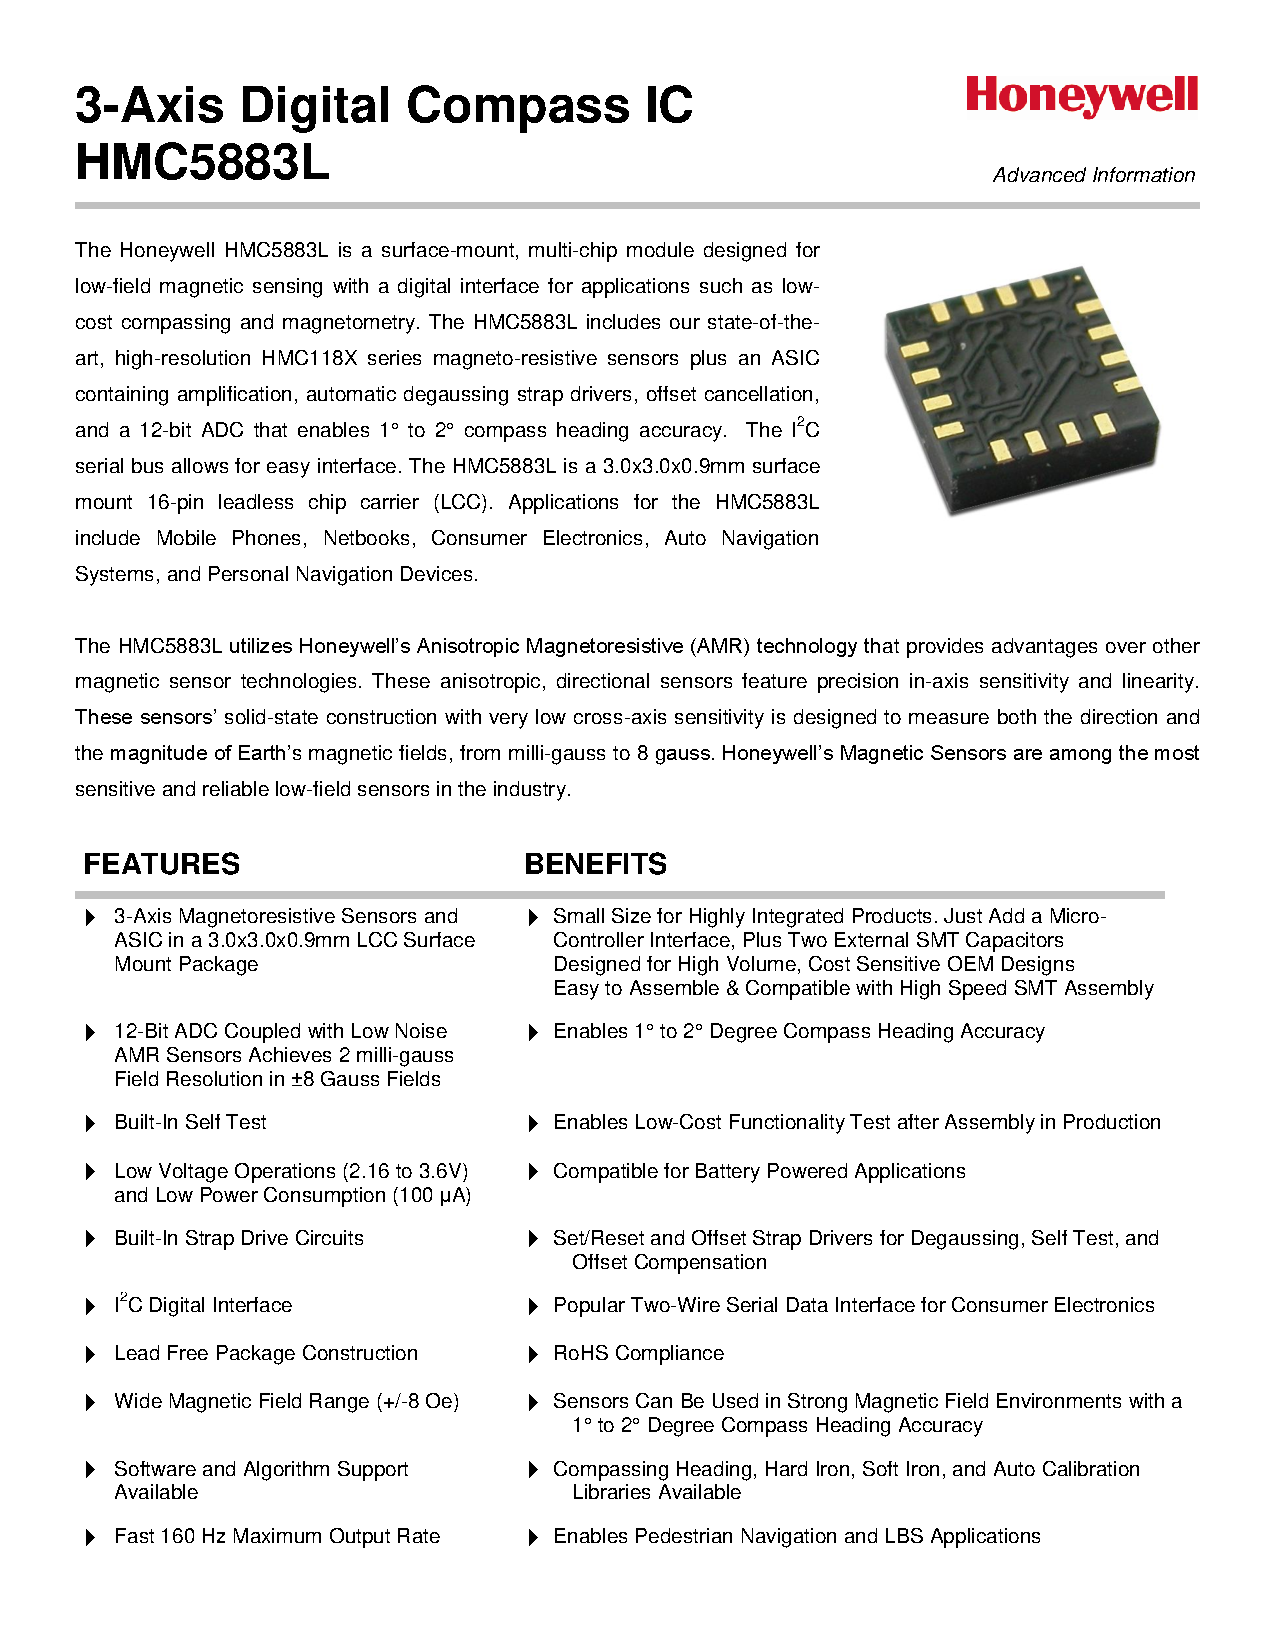
\includepdf[pages=-1]{appendix/mag_px4.pdf}
\chapter{Data Sheets of the x-IMU sensors}\label{ds_ximu}
\includepdf[pages=-1]{appendix/gyro_ximu.pdf}
\includepdf[pages=-1]{appendix/acc_mag_ximu.pdf}


    % uncomment the following line in case you need to make the page wider
    %\addtolength{\headwidth}{1.2cm}\addtolength{\textwidth}{0.5cm}
    %\include{Schematics}
%\end{appendix}
\clear
    %%%%\include{Software}
    % uncomment the following line in case you made the page wider earlier
    %\addtolength{\headwidth}{-1.2cm}\addtolength{\textwidth}{-0.5cm}

\end{document}
